\documentclass[a4paper,12pt]{article}
\usepackage{listings}
\usepackage{graphicx}
\usepackage{epstopdf}
\title{\{M\}assive \{O\}nline \{A\}nalysis Tutorial}
\author{Richard Kirkby}
\date{January 2008}
\begin{document}
\lstset{language=Java,basicstyle=\tiny,numbers=left}

\maketitle

\section{Writing a classifier}

To demonstrate the implementation and operation of learning algorithms in the system, the Java code of a simple decision stump classifier is studied. The classifier monitors the result of splitting on each attribute and chooses the attribute the seems to best separate the classes, based on information gain. The decision is revisited many times, so the stump has potential to change over time as more examples are seen. In practice it is unlikely to change after sufficient training.

To describe the implementation, relevant code fragments are discussed in turn, with the entire code listed (Listing~\ref{lst:fullclassifier}) at the end. The line numbers from the fragments match up with the final listing.

A simple approach to writing a classifier is to extend  \\ \verb+moa.classifiers.AbstractClassifier+ (line 10), which will take care of certain details to ease the task.

\begin{lstlisting}[caption={Option handling},label=lst:opthandle,firstnumber=14]
	public IntOption gracePeriodOption = new IntOption("gracePeriod", 'g',
			"The number of instances to observe between model changes.",
			1000, 0, Integer.MAX_VALUE);

	public FlagOption binarySplitsOption = new FlagOption("binarySplits", 'b',
			"Only allow binary splits.");

	public ClassOption splitCriterionOption = new ClassOption("splitCriterion",
			'c', "Split criterion to use.", SplitCriterion.class,
			"InfoGainSplitCriterion");
\end{lstlisting}

To set up the public interface to the classifier, the options available to the user must be specified. For the system to automatically take care of option handling, the options need to be public members of the class, that extend the \verb+moa.options.Option+ type.

The decision stump classifier example has three options, each of a different type.
The meaning of the first three parameters used to construct options are consistent between different option types. The first parameter is a short name used to identify the option. The second is a character intended to be used on the command line. It should be unique---a command line character cannot be repeated for different options otherwise an exception will be thrown. The third standard parameter is a string describing the purpose of the option. Additional parameters to option constructors allow things such as default values and valid ranges to be specified.

The first option specified for the decision stump classifier is the ``grace period''. The option is expressed with an integer, so the option has the type \verb+IntOption+. The parameter will control how frequently the best stump is reconsidered when learning from a stream of examples. This increases the efficiency of the classifier---evaluating after every single example is expensive, and it is unlikely that a single example will change the decision of the current best stump. The default value of 1000 means that the choice of stump will be re-evaluated only after 1000 examples have been observed since the last evaluation. The last two parameters specify the range of values that are allowed for the option---it makes no sense to have a negative grace period, so the range is restricted to integers 0 or greater.

The second option is a flag, or a binary switch, represented by a \\ \verb+FlagOption+. By default all flags are turned off, and will be turned on only when a user requests so. This flag controls whether the decision stumps should only be allowed to split two ways. By default the stumps are allowed have more than two branches.

The third option determines the split criterion that is used to decide which stumps are the best. This is a \verb+ClassOption+ that requires a particular Java class of the type \verb+SplitCriterion+. If the required class happens to be an \verb+OptionHandler+ then those options will be used to configure the object that is passed in.

\begin{lstlisting}[caption={Miscellaneous fields},label=lst:miscfields,firstnumber=25]
	protected AttributeSplitSuggestion bestSplit;

	protected DoubleVector observedClassDistribution;

	protected AutoExpandVector<AttributeClassObserver> attributeObservers;

	protected double weightSeenAtLastSplit;

	public boolean isRandomizable() {
		return false;
	}
\end{lstlisting}

Four global variables are used to maintain the state of the classifier.

The \verb+bestSplit+ field maintains the current stump that has been chosen by the classifier. It is of type \verb+AttributeSplitSuggestion+, a class used to split instances into different subsets.

The \verb+observedClassDistribution+ field remembers the overall distribution of class labels that have been observed by the classifier. It is of type \verb+DoubleVector+, which is a handy class for maintaining a vector of floating point values without having to manage its size.

The \verb+attributeObservers+ field stores a collection of \\ \verb+AttributeClassObserver+s, one for each attribute. This is the information needed to decide which attribute is best to base the stump on.

The \verb+weightSeenAtLastSplit+ field records the last time an evaluation was performed, so that it can be determined when another evaluation is due, depending on the grace period parameter.

The \verb+isRandomizable()+ function needs to be implemented to specify whether the classifier has an element of randomness. If it does, it will automatically be set up to accept a random seed. This classifier is does not, so \verb+false+ is returned.

\begin{lstlisting}[caption={Preparing for learning},label=lst:preplearn,firstnumber=37]
	@Override
	public void resetLearningImpl() {
		this.bestSplit = null;
		this.observedClassDistribution = new DoubleVector();
		this.attributeObservers = new AutoExpandVector<AttributeClassObserver>();
		this.weightSeenAtLastSplit = 0.0;
	}
\end{lstlisting}

This function is called before any learning begins, so it should set the default state when no information has been supplied, and no training examples have been seen. In this case, the four global fields are set to sensible defaults.

\begin{lstlisting}[caption={Training on examples},label=lst:train,firstnumber=45]
	@Override
	public void trainOnInstanceImpl(Instance inst) {
		this.observedClassDistribution.addToValue((int) inst.classValue(), inst
				.weight());
		for (int i = 0; i < inst.numAttributes() - 1; i++) {
			int instAttIndex = modelAttIndexToInstanceAttIndex(i, inst);
			AttributeClassObserver obs = this.attributeObservers.get(i);
			if (obs == null) {
				obs = inst.attribute(instAttIndex).isNominal() ?
					newNominalClassObserver() : newNumericClassObserver();
				this.attributeObservers.set(i, obs);
			}
			obs.observeAttributeClass(inst.value(instAttIndex), (int) inst
					.classValue(), inst.weight());
		}
		if (this.trainingWeightSeenByModel - this.weightSeenAtLastSplit >=
				this.gracePeriodOption.getValue()) {
			this.bestSplit = findBestSplit((SplitCriterion)
				getPreparedClassOption(this.splitCriterionOption));
			this.weightSeenAtLastSplit = this.trainingWeightSeenByModel;
		}
	}
\end{lstlisting}

This is the main function of the learning algorithm, called for every training example in a stream. The first step, lines 47-48, updates the overall recorded distribution of classes. The loop from line 49 to line 59 repeats for every attribute in the data. If no observations for a particular attribute have been seen previously, then lines 53-55 create a new observing object. Lines 57-58 update the observations with the values from the new example. Lines 60-61 check to see if the grace period has expired. If so, the best split is re-evaluated.

\begin{lstlisting}[caption={Functions used during training},label=lst:trainfuncs,firstnumber=79]
	protected AttributeClassObserver newNominalClassObserver() {
		return new NominalAttributeClassObserver();
	}

	protected AttributeClassObserver newNumericClassObserver() {
		return new GaussianNumericAttributeClassObserver();
	}

	protected AttributeSplitSuggestion findBestSplit(SplitCriterion criterion) {
		AttributeSplitSuggestion bestFound = null;
		double bestMerit = Double.NEGATIVE_INFINITY;
		double[] preSplitDist = this.observedClassDistribution.getArrayCopy();
		for (int i = 0; i < this.attributeObservers.size(); i++) {
			AttributeClassObserver obs = this.attributeObservers.get(i);
			if (obs != null) {
				AttributeSplitSuggestion suggestion =
					obs.getBestEvaluatedSplitSuggestion(
						criterion,
						preSplitDist,
						i,
						this.binarySplitsOption.isSet());
				if (suggestion.merit > bestMerit) {
					bestMerit = suggestion.merit;
					bestFound = suggestion;
				}
			}
		}
		return bestFound;
	}
\end{lstlisting}

These functions assist the training algorithm. \\ \verb+newNominalClassObserver+ and \verb+newNumericClassObserver+ are responsible for creating new observer objects for nominal and numeric attributes, respectively. The \verb+findBestSplit()+ function will iterate through the possible stumps and return the one with the highest `merit' score.

\begin{lstlisting}[caption={Predicting class of unknown examples},label=lst:test,firstnumber=68]
	public double[] getVotesForInstance(Instance inst) {
		if (this.bestSplit != null) {
			int branch = this.bestSplit.splitTest.branchForInstance(inst);
			if (branch >= 0) {
				return this.bestSplit
						.resultingClassDistributionFromSplit(branch);
			}
		}
		return this.observedClassDistribution.getArrayCopy();
	}
\end{lstlisting}

This is the other important function of the classifier besides training---using the model that has been induced to predict the class of examples. For the decision stump, this involves calling the functions \verb+branchForInstance()+ and \verb+resultingClassDistributionFromSplit()+ that are implemented by the \verb+AttributeSplitSuggestion+ class.

Putting all of the elements together, the full listing of the tutorial class is given below.

\begin{lstlisting}[caption={Full listing},label=lst:fullclassifier]
package moa.classifiers;

import moa.core.AutoExpandVector;
import moa.core.DoubleVector;
import moa.options.ClassOption;
import moa.options.FlagOption;
import moa.options.IntOption;
import weka.core.Instance;

public class DecisionStumpTutorial extends AbstractClassifier {

	private static final long serialVersionUID = 1L;

	public IntOption gracePeriodOption = new IntOption("gracePeriod", 'g',
			"The number of instances to observe between model changes.",
			1000, 0, Integer.MAX_VALUE);

	public FlagOption binarySplitsOption = new FlagOption("binarySplits", 'b',
			"Only allow binary splits.");

	public ClassOption splitCriterionOption = new ClassOption("splitCriterion",
			'c', "Split criterion to use.", SplitCriterion.class,
			"InfoGainSplitCriterion");

	protected AttributeSplitSuggestion bestSplit;

	protected DoubleVector observedClassDistribution;

	protected AutoExpandVector<AttributeClassObserver> attributeObservers;

	protected double weightSeenAtLastSplit;

	public boolean isRandomizable() {
		return false;
	}

	@Override
	public void resetLearningImpl() {
		this.bestSplit = null;
		this.observedClassDistribution = new DoubleVector();
		this.attributeObservers = new AutoExpandVector<AttributeClassObserver>();
		this.weightSeenAtLastSplit = 0.0;
	}

	@Override
	public void trainOnInstanceImpl(Instance inst) {
		this.observedClassDistribution.addToValue((int) inst.classValue(), inst
				.weight());
		for (int i = 0; i < inst.numAttributes() - 1; i++) {
			int instAttIndex = modelAttIndexToInstanceAttIndex(i, inst);
			AttributeClassObserver obs = this.attributeObservers.get(i);
			if (obs == null) {
				obs = inst.attribute(instAttIndex).isNominal() ?
					newNominalClassObserver() : newNumericClassObserver();
				this.attributeObservers.set(i, obs);
			}
			obs.observeAttributeClass(inst.value(instAttIndex), (int) inst
					.classValue(), inst.weight());
		}
		if (this.trainingWeightSeenByModel - this.weightSeenAtLastSplit >=
				this.gracePeriodOption.getValue()) {
			this.bestSplit = findBestSplit((SplitCriterion)
				getPreparedClassOption(this.splitCriterionOption));
			this.weightSeenAtLastSplit = this.trainingWeightSeenByModel;
		}
	}

	public double[] getVotesForInstance(Instance inst) {
		if (this.bestSplit != null) {
			int branch = this.bestSplit.splitTest.branchForInstance(inst);
			if (branch >= 0) {
				return this.bestSplit
						.resultingClassDistributionFromSplit(branch);
			}
		}
		return this.observedClassDistribution.getArrayCopy();
	}

	protected AttributeClassObserver newNominalClassObserver() {
		return new NominalAttributeClassObserver();
	}

	protected AttributeClassObserver newNumericClassObserver() {
		return new GaussianNumericAttributeClassObserver();
	}

	protected AttributeSplitSuggestion findBestSplit(SplitCriterion criterion) {
		AttributeSplitSuggestion bestFound = null;
		double bestMerit = Double.NEGATIVE_INFINITY;
		double[] preSplitDist = this.observedClassDistribution.getArrayCopy();
		for (int i = 0; i < this.attributeObservers.size(); i++) {
			AttributeClassObserver obs = this.attributeObservers.get(i);
			if (obs != null) {
				AttributeSplitSuggestion suggestion =
					obs.getBestEvaluatedSplitSuggestion(
						criterion,
						preSplitDist,
						i,
						this.binarySplitsOption.isSet());
				if (suggestion.merit > bestMerit) {
					bestMerit = suggestion.merit;
					bestFound = suggestion;
				}
			}
		}
		return bestFound;
	}

	public void getModelDescription(StringBuilder out, int indent) {
	}

	protected moa.core.Measurement[] getModelMeasurementsImpl() {
		return null;
	}

}
\end{lstlisting}

\section{Using the command line}

The following examples are based on a Unix/Linux system with Java 5 SDK or greater installed. Other operating systems such as Microsoft Windows will be similar but may need adjustments to suit.

The following five files are assumed to be in the current working directory:

\begin{verbatim}
DecisionStumpTutorial.java
moa.jar
weka.jar
sizeofag.jar
\end{verbatim}

The example source code can be compiled with the following command:

\begin{verbatim}
javac -cp moa.jar:weka.jar DecisionStumpTutorial.java
\end{verbatim}

This produces compiled java class file \verb+DecisionStumpTutorial.class+.

Before continuing, the commands below set up directory structure to reflect the package structure:

\begin{verbatim}
mkdir moa
mkdir moa/classifiers
cp DecisionStumpTutorial.class moa/classifiers/
\end{verbatim}

The class is now ready to use.

The first example will command MOA to train the \verb+DecisionStumpTutorial+ classifier and create a model. The \verb+moa.DoTask+ class is the main class for running tasks on the command line. It will accept the name of a task followed by any appropriate parameters. The first task used is the \verb+LearnModel+ task. The \verb+-l+ parameter specifies the learner, in this case the \verb+DecisionStumpTutorial+ class. The \verb+-s+ parameter specifies the stream to learn from, in this case \verb+generators.WaveformGenerator+ is specified, which is a data stream generator that produces a three-class learning problem of identifying three types of waveform. The \verb+-m+ option specifies the maximum number of examples to train the learner with, in this case one million examples. The \verb+-O+ option specifies a file to output the resulting model to:

\begin{verbatim}
java -cp .:moa.jar:weka.jar -javaagent:sizeofag.jar moa.DoTask \
  LearnModel -l DecisionStumpTutorial \
  -s generators.WaveformGenerator -m 1000000 -O model1.moa
\end{verbatim}

This will create a file named \verb+model1.moa+ that contains the decision stump model that was induced during training.

The next example will evaluate the model to see how accurate it is on a set of examples that are generated using a different random seed. The \verb+EvaluateModel+ task is given the parameters needed to load the model produced in the previous step, generate a new waveform stream with a random seed of 2, and test on one million examples:

\begin{verbatim}
java -cp .:moa.jar:weka.jar -javaagent:sizeofag.jar moa.DoTask \
  "EvaluateModel -m file:model1.moa \
  -s (generators.WaveformGenerator -i 2) -i 1000000"
\end{verbatim}

This is the first example of nesting parameters using brackets. Quotes have been added around the description of the task, otherwise the operating system may be confused about the meaning of the brackets.

After evaluation the following statistics are output:

\begin{verbatim}
classified instances = 1,000,000
classifications correct (percent) = 57.637
\end{verbatim}

Note the the above two steps can be achieved by rolling them into one, avoiding the need to create an external file, as follows:

\begin{verbatim}
java -cp .:moa.jar:weka.jar -javaagent:sizeofag.jar moa.DoTask \
  "EvaluateModel -m (LearnModel -l DecisionStumpTutorial \
  -s generators.WaveformGenerator -m 1000000) \
  -s (generators.WaveformGenerator -i 2) -i 1000000"
\end{verbatim}

The task \verb+EvaluatePeriodicHeldOutTest+ will train a model while taking snapshots of performance using a held-out test set at periodic intervals.
The following command creates a {\em comma separated values} file, training the \verb+DecisionStumpTutorial+ classifier on the \verb+WaveformGenerator+ data, using the first 100 thousand examples for testing, training on a total of 100 million examples, and testing every one million examples:

\begin{verbatim}
java -cp .:moa.jar:weka.jar -javaagent:sizeofag.jar moa.DoTask \
  "EvaluatePeriodicHeldOutTest -l DecisionStumpTutorial \
  -s generators.WaveformGenerator \
  -n 100000 -i 10000000 -f 1000000" > dsresult.csv
\end{verbatim}

For the purposes of comparison, a decision tree learner can be trained on the same problem:

\begin{verbatim}
java -cp .:moa.jar:weka.jar -javaagent:sizeofag.jar moa.DoTask \
  "EvaluatePeriodicHeldOutTest -l HoeffdingTree \
  -s generators.WaveformGenerator \
  -n 100000 -i 10000000 -f 1000000" > htresult.csv
\end{verbatim}

Assuming that \verb+gnuplot+ is installed on the system, the learning curves can be plotted with the following commands:

\begin{verbatim}
gnuplot> set datafile separator ","
gnuplot> set ylabel "% correct"
gnuplot> set xlabel "examples processed"
gnuplot> plot [][0:100] \
  "dsresult.csv" using 1:9 with linespoints \
  title "DecisionStumpTutorial", \
  "htresult.csv" using 1:9 with linespoints \
  title "HoeffdingTree"
\end{verbatim}

This results in the following graph:

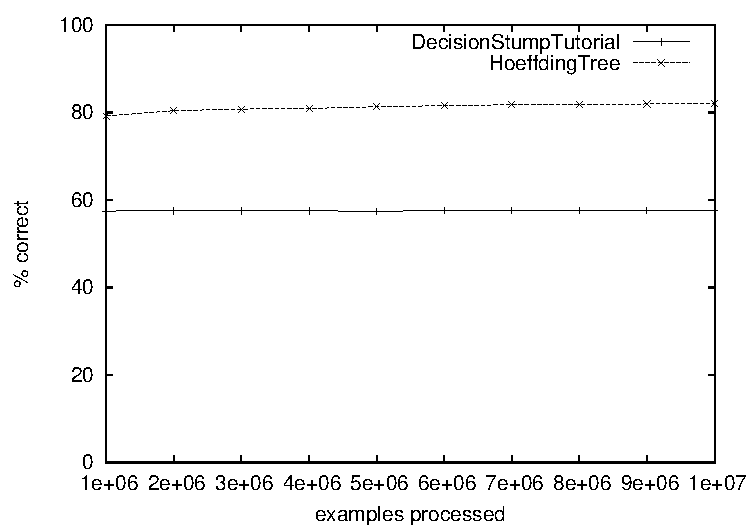
\includegraphics{gnuplotGraph}

For this problem it is obvious that a full tree can achieve higher accuracy than a single stump, and that a stump has very stable accuracy that does not improve with further training.

\section{Using the GUI}

Start a graphical user interface for configuring and running tasks with the command:

\begin{verbatim}
java -cp .:moa.jar:weka.jar -javaagent:sizeofag.jar \
  moa.gui.TaskLauncher
\end{verbatim}

Click 'Configure' to set up a task, when ready click to launch a task click 'Run'. Several tasks can be run concurrently. Click on different tasks in the list and control them using the buttons below. If textual output of a task is available it will be displayed in the bottom half of the GUI, and can be saved to disk.

Note that the command line text box displayed at the top of the window represents textual commands that can be used to run tasks on the command line as described in the previous section. The text can be selected then copied onto the clipboard. 

\end{document}